\section{Application de téléversement}\label{sec:application-de-téléversement}

    \subsection{Prérequis et Intallation}\label{subsec:prerequis-et-intallation}

        \begin{figure}[H]
            \begin{center}
                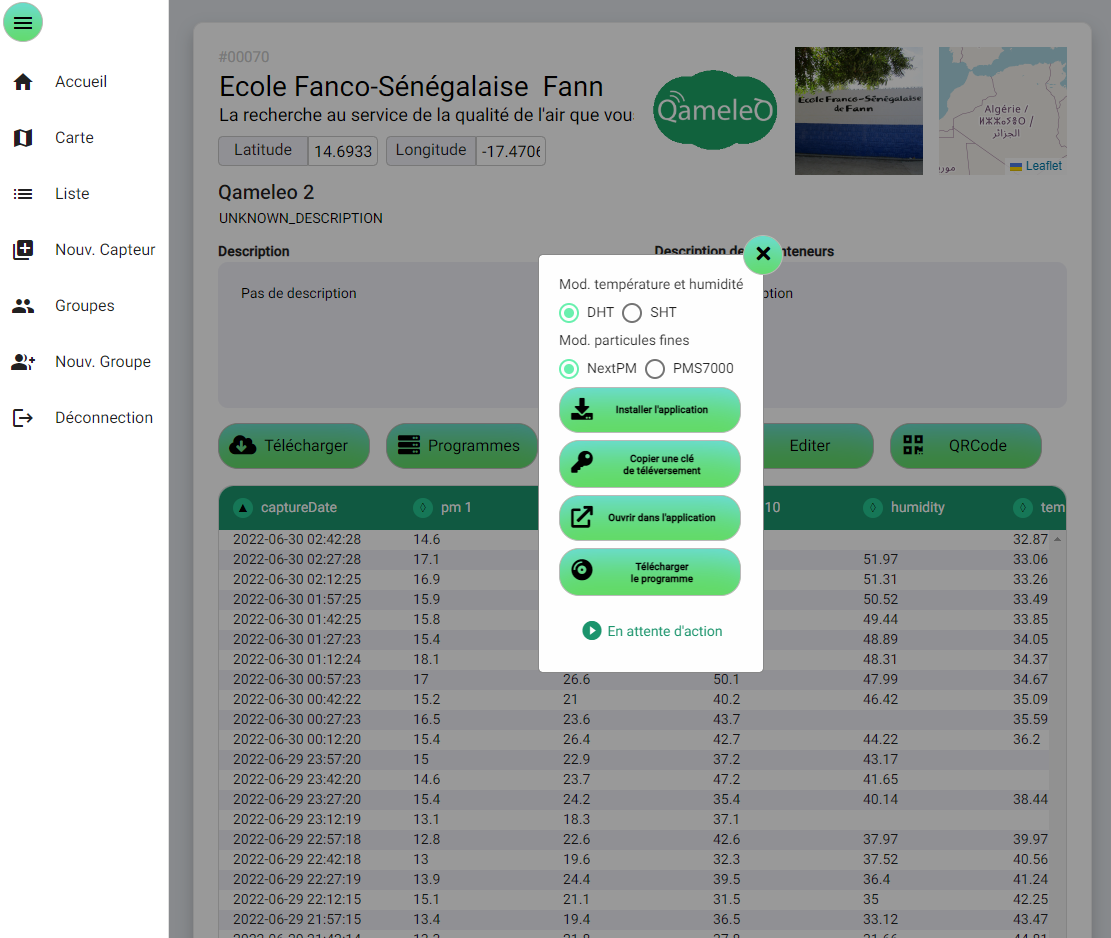
\includegraphics[width=12cm]{resources/sensor_app}
            \end{center}
            \caption{Page de l'application}\label{fig:page-de-l-application}
        \end{figure}

        Afin de permettre l'interaction entre le site web et l'Arduino, une application de bureau a été développée.
        Cette application est récupérable à partir de n'importe quel capteur en appuyant sur ``Programmes'' puis ``Installer l'application''.
        Vous récupérez alors une JAR, un programme utilisant java pour fonctionner.
        Si vous n'avez pas java installer, merci de suivre les indications sur \href{https://www.java.com}{www.java.com}.
        Une fois que vous lancez l'application, vous aurez un avertissement vous demandant une ``installation privilégié''
        si vous souhaitez utiliser pleinement les fonctionnalités fournies par windows (Ouverture de fichier et lancement de l'application depuis un navigateur).
        Suite à cela l'installation sera terminée.
        À noter qu'elle vous sera automatiquement redemandée si vous déplacer l'application.

    \subsection{Utilisation}\label{subsec:utilisation}

        \begin{figure}[H]
            \begin{center}
                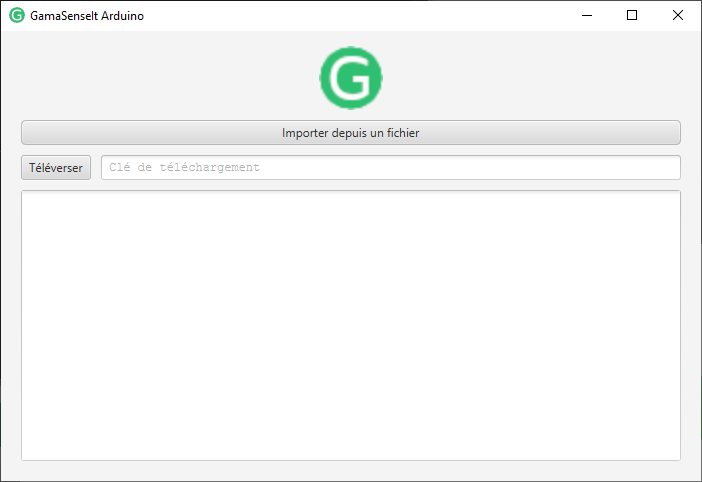
\includegraphics[width=12cm]{resources/app}
            \end{center}
            \caption{Application de téléversement}\label{fig:app-televersement}
        \end{figure}

        Sur cette application vous aurez 3 possibilités pour téléverser le programme d'un capteur :

        \begin{itemize}
            \item Via une clé de téléchargement
            \item En l'ouvrant depuis le navigateur (Windows seulement)
            \item En téléchargent le fichier (Windows et partiellement sur les autres)
        \end{itemize}

        \subsubsection{Téléversement par clé}

            Vous pouvez utiliser une clé que vous récupérer en cliquant sur ``copier une clé de téléversement''.
            Cette clé est alors valide pendant 15 min.
            Suite à cela, copier la clé dans le champ ``Clé de téléchargement'' puis appuyez sur ``Téléverser''.
            Il vous sera demandé de confirmer le télécharmeent et optionnellement, si le site ne support pas le https,
            de téléchargement de façons non sécurisé.

        \subsubsection{Téléversement par navigateur}

            Si vous êtes sur windows et avez suivi les étapes précédents vous pouvez appuier sur ``Ouvrir dans l'application''
            sur le site web puis confirmé sur l'application telle que précédament.

        \subsubsection{Téléversement par fichier}

            Pour procédé au téléversement en passant par un fichier, il faut tout d'abors télécharger le fichier
            en appuyant sur Télécharger le programme puis en sélectionnant la destination.
            Une fois ceci faites-vous pouvez directement ouvrir le fichier en cliquant dessus si l'application
            et correctement installer et que vous êtes sur une machine Windows.
            Dans le cas contraire vous pouvez ouvrir l'application puis appuyée sur ``Importer depuis un fichier'',
            puis sélectionner votre fichier et confirmer.

        \subsection{Moniteur Serial}\label{subsec:moniteur-serial}

            De plus l'application possède un moniteur serial permettant de voir les sorties du programme en temps réel.
